\begin{figure*}[htbp]
  \centering
  % 第一部分 (a) - 左侧
  \begin{subfigure}{0.48\linewidth}
    \centering
    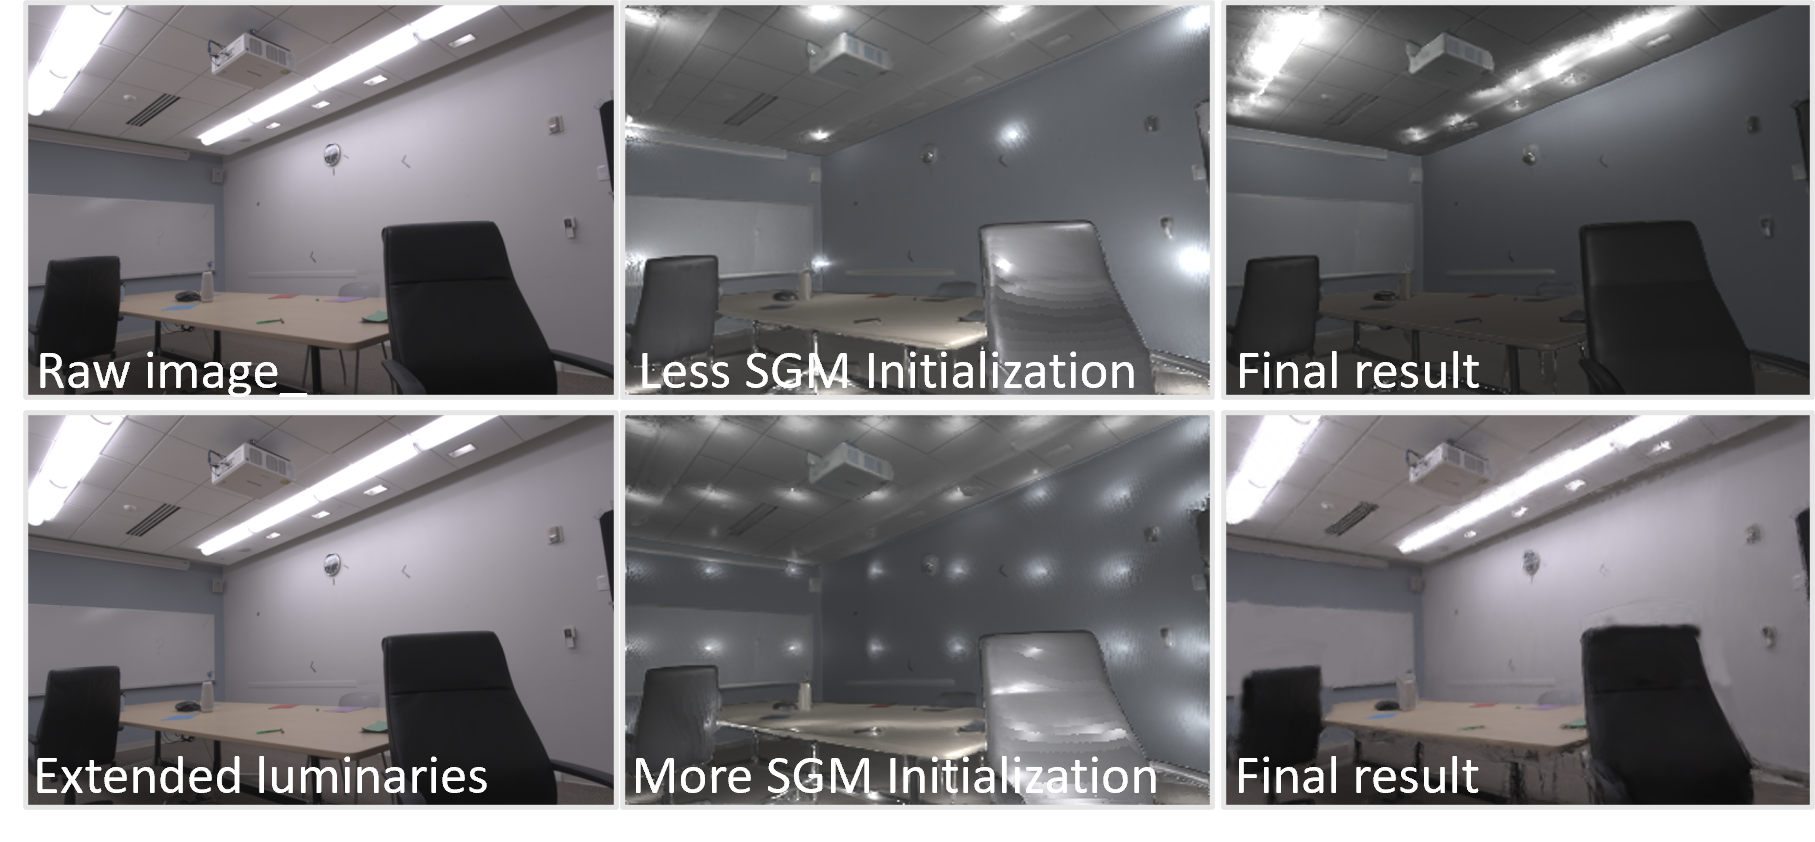
\includegraphics[width=\linewidth]{images/extend_luminaries.png}
    \vspace{-6mm} 
    \label{fig:light_source}
  \end{subfigure}%
  \hspace{1.5mm}
  % --- 中间的灰色虚线 ---
  \begin{tikzpicture}
    \draw[dash pattern=on 3pt off 3pt, gray!50, thick] (0,0) -- (0,3.5cm); % 3.5cm为高度，可根据图片高度手动微调
  \end{tikzpicture}
  \hspace{0.1mm}
  % 第二部分 (b) - 右侧
  \begin{subfigure}{0.48\linewidth}
    \centering
    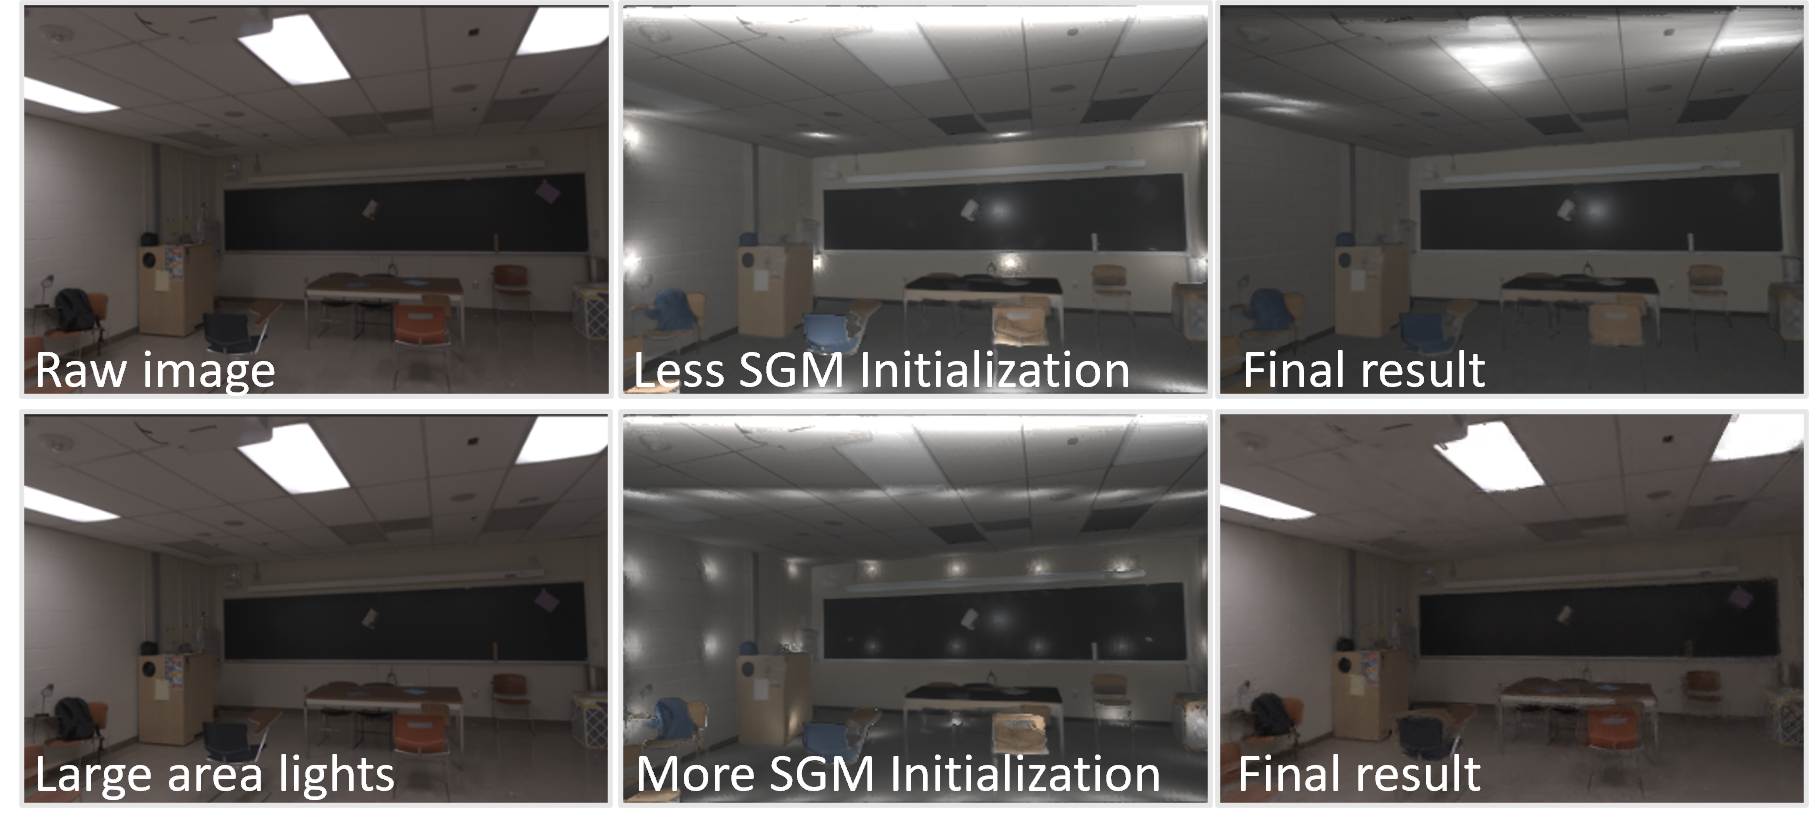
\includegraphics[width=\linewidth]{images/large_area_lights.png}
    \vspace{-6.1mm}
    \label{fig:scene_composition}
  \end{subfigure}
  \vspace{-1mm}
  \caption{\textbf{Expressiveness of our SGM-based interior lighting model for complex emitters.}}
  \label{fig:complex_emitter}
\end{figure*}